% Created by tikzDevice version 0.12.3.1 on 2023-04-24 13:44:38
% !TEX encoding = UTF-8 Unicode
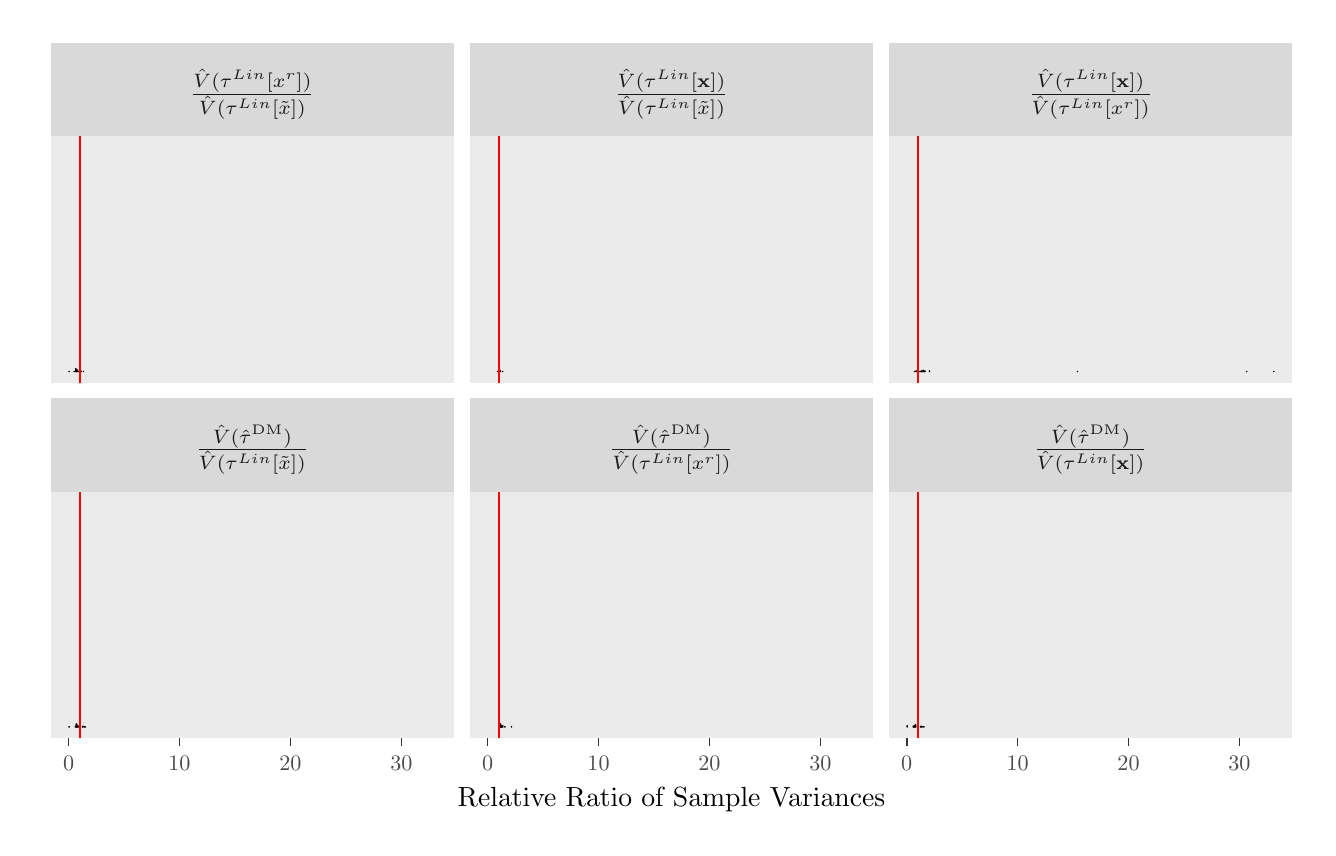
\begin{tikzpicture}[x=1pt,y=1pt]
\definecolor{fillColor}{RGB}{255,255,255}
\path[use as bounding box,fill=fillColor,fill opacity=0.00] (0,0) rectangle (462.53,289.08);
\begin{scope}
\path[clip] (  0.00,  0.00) rectangle (462.53,289.08);
\definecolor{drawColor}{RGB}{255,255,255}
\definecolor{fillColor}{RGB}{255,255,255}

\path[draw=drawColor,line width= 0.6pt,line join=round,line cap=round,fill=fillColor] (  0.00,  0.00) rectangle (462.53,289.08);
\end{scope}
\begin{scope}
\path[clip] (  8.25,160.68) rectangle (154.18,249.78);
\definecolor{fillColor}{gray}{0.92}

\path[fill=fillColor] (  8.25,160.68) rectangle (154.18,249.78);
\definecolor{drawColor}{RGB}{0,0,0}
\definecolor{fillColor}{RGB}{0,0,0}

\path[draw=drawColor,line width= 0.4pt,line join=round,fill=fillColor] ( 14.98,164.83) circle (  0.10);

\path[draw=drawColor,line width= 0.4pt,line join=round,fill=fillColor] ( 16.79,164.83) circle (  0.10);

\path[draw=drawColor,line width= 0.4pt,line join=round,fill=fillColor] ( 17.39,164.83) circle (  0.10);

\path[draw=drawColor,line width= 0.4pt,line join=round,fill=fillColor] ( 17.39,165.03) circle (  0.10);

\path[draw=drawColor,line width= 0.4pt,line join=round,fill=fillColor] ( 17.39,165.23) circle (  0.10);

\path[draw=drawColor,line width= 0.4pt,line join=round,fill=fillColor] ( 17.39,165.43) circle (  0.10);

\path[draw=drawColor,line width= 0.4pt,line join=round,fill=fillColor] ( 17.39,165.63) circle (  0.10);

\path[draw=drawColor,line width= 0.4pt,line join=round,fill=fillColor] ( 17.39,165.83) circle (  0.10);

\path[draw=drawColor,line width= 0.4pt,line join=round,fill=fillColor] ( 17.59,164.83) circle (  0.10);

\path[draw=drawColor,line width= 0.4pt,line join=round,fill=fillColor] ( 17.59,165.03) circle (  0.10);

\path[draw=drawColor,line width= 0.4pt,line join=round,fill=fillColor] ( 17.59,165.23) circle (  0.10);

\path[draw=drawColor,line width= 0.4pt,line join=round,fill=fillColor] ( 17.79,164.83) circle (  0.10);

\path[draw=drawColor,line width= 0.4pt,line join=round,fill=fillColor] ( 17.79,165.03) circle (  0.10);

\path[draw=drawColor,line width= 0.4pt,line join=round,fill=fillColor] ( 17.79,165.23) circle (  0.10);

\path[draw=drawColor,line width= 0.4pt,line join=round,fill=fillColor] ( 17.79,165.43) circle (  0.10);

\path[draw=drawColor,line width= 0.4pt,line join=round,fill=fillColor] ( 17.99,164.83) circle (  0.10);

\path[draw=drawColor,line width= 0.4pt,line join=round,fill=fillColor] ( 18.19,164.83) circle (  0.10);

\path[draw=drawColor,line width= 0.4pt,line join=round,fill=fillColor] ( 18.39,164.83) circle (  0.10);

\path[draw=drawColor,line width= 0.4pt,line join=round,fill=fillColor] ( 18.59,164.83) circle (  0.10);

\path[draw=drawColor,line width= 0.4pt,line join=round,fill=fillColor] ( 19.19,164.83) circle (  0.10);

\path[draw=drawColor,line width= 0.4pt,line join=round,fill=fillColor] ( 19.19,165.03) circle (  0.10);

\path[draw=drawColor,line width= 0.4pt,line join=round,fill=fillColor] ( 19.39,164.83) circle (  0.10);

\path[draw=drawColor,line width= 0.4pt,line join=round,fill=fillColor] ( 20.19,164.83) circle (  0.10);
\definecolor{drawColor}{RGB}{255,0,0}

\path[draw=drawColor,line width= 0.6pt,line join=round] ( 18.79,160.68) -- ( 18.79,249.78);
\end{scope}
\begin{scope}
\path[clip] (  8.25, 32.28) rectangle (154.18,121.38);
\definecolor{fillColor}{gray}{0.92}

\path[fill=fillColor] (  8.25, 32.28) rectangle (154.18,121.38);
\definecolor{drawColor}{RGB}{0,0,0}
\definecolor{fillColor}{RGB}{0,0,0}

\path[draw=drawColor,line width= 0.4pt,line join=round,fill=fillColor] ( 14.98, 36.43) circle (  0.10);

\path[draw=drawColor,line width= 0.4pt,line join=round,fill=fillColor] ( 17.19, 36.43) circle (  0.10);

\path[draw=drawColor,line width= 0.4pt,line join=round,fill=fillColor] ( 17.59, 36.43) circle (  0.10);

\path[draw=drawColor,line width= 0.4pt,line join=round,fill=fillColor] ( 17.59, 36.63) circle (  0.10);

\path[draw=drawColor,line width= 0.4pt,line join=round,fill=fillColor] ( 17.59, 36.83) circle (  0.10);

\path[draw=drawColor,line width= 0.4pt,line join=round,fill=fillColor] ( 17.59, 37.03) circle (  0.10);

\path[draw=drawColor,line width= 0.4pt,line join=round,fill=fillColor] ( 17.59, 37.23) circle (  0.10);

\path[draw=drawColor,line width= 0.4pt,line join=round,fill=fillColor] ( 17.59, 37.43) circle (  0.10);

\path[draw=drawColor,line width= 0.4pt,line join=round,fill=fillColor] ( 17.79, 36.43) circle (  0.10);

\path[draw=drawColor,line width= 0.4pt,line join=round,fill=fillColor] ( 17.79, 36.63) circle (  0.10);

\path[draw=drawColor,line width= 0.4pt,line join=round,fill=fillColor] ( 17.99, 36.43) circle (  0.10);

\path[draw=drawColor,line width= 0.4pt,line join=round,fill=fillColor] ( 17.99, 36.63) circle (  0.10);

\path[draw=drawColor,line width= 0.4pt,line join=round,fill=fillColor] ( 17.99, 36.83) circle (  0.10);

\path[draw=drawColor,line width= 0.4pt,line join=round,fill=fillColor] ( 17.99, 37.03) circle (  0.10);

\path[draw=drawColor,line width= 0.4pt,line join=round,fill=fillColor] ( 18.19, 36.43) circle (  0.10);

\path[draw=drawColor,line width= 0.4pt,line join=round,fill=fillColor] ( 18.59, 36.43) circle (  0.10);

\path[draw=drawColor,line width= 0.4pt,line join=round,fill=fillColor] ( 18.59, 36.63) circle (  0.10);

\path[draw=drawColor,line width= 0.4pt,line join=round,fill=fillColor] ( 18.99, 36.43) circle (  0.10);

\path[draw=drawColor,line width= 0.4pt,line join=round,fill=fillColor] ( 19.79, 36.43) circle (  0.10);

\path[draw=drawColor,line width= 0.4pt,line join=round,fill=fillColor] ( 19.99, 36.43) circle (  0.10);

\path[draw=drawColor,line width= 0.4pt,line join=round,fill=fillColor] ( 19.99, 36.63) circle (  0.10);

\path[draw=drawColor,line width= 0.4pt,line join=round,fill=fillColor] ( 20.59, 36.43) circle (  0.10);

\path[draw=drawColor,line width= 0.4pt,line join=round,fill=fillColor] ( 20.79, 36.43) circle (  0.10);
\definecolor{drawColor}{RGB}{255,0,0}

\path[draw=drawColor,line width= 0.6pt,line join=round] ( 18.79, 32.28) -- ( 18.79,121.38);
\end{scope}
\begin{scope}
\path[clip] (159.68,160.68) rectangle (305.60,249.78);
\definecolor{fillColor}{gray}{0.92}

\path[fill=fillColor] (159.68,160.68) rectangle (305.60,249.78);
\definecolor{drawColor}{RGB}{0,0,0}
\definecolor{fillColor}{RGB}{0,0,0}

\path[draw=drawColor,line width= 0.4pt,line join=round,fill=fillColor] (169.82,164.83) circle (  0.10);

\path[draw=drawColor,line width= 0.4pt,line join=round,fill=fillColor] (170.02,164.83) circle (  0.10);

\path[draw=drawColor,line width= 0.4pt,line join=round,fill=fillColor] (170.22,164.83) circle (  0.10);

\path[draw=drawColor,line width= 0.4pt,line join=round,fill=fillColor] (170.22,165.03) circle (  0.10);

\path[draw=drawColor,line width= 0.4pt,line join=round,fill=fillColor] (170.22,165.23) circle (  0.10);

\path[draw=drawColor,line width= 0.4pt,line join=round,fill=fillColor] (170.22,165.43) circle (  0.10);

\path[draw=drawColor,line width= 0.4pt,line join=round,fill=fillColor] (170.22,165.63) circle (  0.10);

\path[draw=drawColor,line width= 0.4pt,line join=round,fill=fillColor] (170.22,165.83) circle (  0.10);

\path[draw=drawColor,line width= 0.4pt,line join=round,fill=fillColor] (170.22,166.03) circle (  0.10);

\path[draw=drawColor,line width= 0.4pt,line join=round,fill=fillColor] (170.22,166.23) circle (  0.10);

\path[draw=drawColor,line width= 0.4pt,line join=round,fill=fillColor] (170.22,166.43) circle (  0.10);

\path[draw=drawColor,line width= 0.4pt,line join=round,fill=fillColor] (170.22,166.63) circle (  0.10);

\path[draw=drawColor,line width= 0.4pt,line join=round,fill=fillColor] (170.22,166.83) circle (  0.10);

\path[draw=drawColor,line width= 0.4pt,line join=round,fill=fillColor] (170.22,167.03) circle (  0.10);

\path[draw=drawColor,line width= 0.4pt,line join=round,fill=fillColor] (170.22,167.23) circle (  0.10);

\path[draw=drawColor,line width= 0.4pt,line join=round,fill=fillColor] (170.42,164.83) circle (  0.10);

\path[draw=drawColor,line width= 0.4pt,line join=round,fill=fillColor] (170.42,165.03) circle (  0.10);

\path[draw=drawColor,line width= 0.4pt,line join=round,fill=fillColor] (170.42,165.23) circle (  0.10);

\path[draw=drawColor,line width= 0.4pt,line join=round,fill=fillColor] (170.62,164.83) circle (  0.10);

\path[draw=drawColor,line width= 0.4pt,line join=round,fill=fillColor] (170.62,165.03) circle (  0.10);

\path[draw=drawColor,line width= 0.4pt,line join=round,fill=fillColor] (170.62,165.23) circle (  0.10);

\path[draw=drawColor,line width= 0.4pt,line join=round,fill=fillColor] (170.82,164.83) circle (  0.10);

\path[draw=drawColor,line width= 0.4pt,line join=round,fill=fillColor] (171.62,164.83) circle (  0.10);
\definecolor{drawColor}{RGB}{255,0,0}

\path[draw=drawColor,line width= 0.6pt,line join=round] (170.22,160.68) -- (170.22,249.78);
\end{scope}
\begin{scope}
\path[clip] (159.68, 32.28) rectangle (305.60,121.38);
\definecolor{fillColor}{gray}{0.92}

\path[fill=fillColor] (159.68, 32.28) rectangle (305.60,121.38);
\definecolor{drawColor}{RGB}{0,0,0}
\definecolor{fillColor}{RGB}{0,0,0}

\path[draw=drawColor,line width= 0.4pt,line join=round,fill=fillColor] (170.22, 36.43) circle (  0.10);

\path[draw=drawColor,line width= 0.4pt,line join=round,fill=fillColor] (170.22, 36.63) circle (  0.10);

\path[draw=drawColor,line width= 0.4pt,line join=round,fill=fillColor] (170.22, 36.83) circle (  0.10);

\path[draw=drawColor,line width= 0.4pt,line join=round,fill=fillColor] (170.22, 37.03) circle (  0.10);

\path[draw=drawColor,line width= 0.4pt,line join=round,fill=fillColor] (170.22, 37.23) circle (  0.10);

\path[draw=drawColor,line width= 0.4pt,line join=round,fill=fillColor] (170.42, 36.43) circle (  0.10);

\path[draw=drawColor,line width= 0.4pt,line join=round,fill=fillColor] (170.42, 36.63) circle (  0.10);

\path[draw=drawColor,line width= 0.4pt,line join=round,fill=fillColor] (170.42, 36.83) circle (  0.10);

\path[draw=drawColor,line width= 0.4pt,line join=round,fill=fillColor] (170.42, 37.03) circle (  0.10);

\path[draw=drawColor,line width= 0.4pt,line join=round,fill=fillColor] (170.42, 37.23) circle (  0.10);

\path[draw=drawColor,line width= 0.4pt,line join=round,fill=fillColor] (170.62, 36.43) circle (  0.10);

\path[draw=drawColor,line width= 0.4pt,line join=round,fill=fillColor] (170.62, 36.63) circle (  0.10);

\path[draw=drawColor,line width= 0.4pt,line join=round,fill=fillColor] (170.62, 36.83) circle (  0.10);

\path[draw=drawColor,line width= 0.4pt,line join=round,fill=fillColor] (170.62, 37.03) circle (  0.10);

\path[draw=drawColor,line width= 0.4pt,line join=round,fill=fillColor] (170.62, 37.23) circle (  0.10);

\path[draw=drawColor,line width= 0.4pt,line join=round,fill=fillColor] (170.62, 37.43) circle (  0.10);

\path[draw=drawColor,line width= 0.4pt,line join=round,fill=fillColor] (170.62, 37.63) circle (  0.10);

\path[draw=drawColor,line width= 0.4pt,line join=round,fill=fillColor] (170.82, 36.43) circle (  0.10);

\path[draw=drawColor,line width= 0.4pt,line join=round,fill=fillColor] (170.82, 36.63) circle (  0.10);

\path[draw=drawColor,line width= 0.4pt,line join=round,fill=fillColor] (170.82, 36.83) circle (  0.10);

\path[draw=drawColor,line width= 0.4pt,line join=round,fill=fillColor] (170.82, 37.03) circle (  0.10);

\path[draw=drawColor,line width= 0.4pt,line join=round,fill=fillColor] (170.82, 37.23) circle (  0.10);

\path[draw=drawColor,line width= 0.4pt,line join=round,fill=fillColor] (171.02, 36.43) circle (  0.10);

\path[draw=drawColor,line width= 0.4pt,line join=round,fill=fillColor] (171.02, 36.63) circle (  0.10);

\path[draw=drawColor,line width= 0.4pt,line join=round,fill=fillColor] (171.02, 36.83) circle (  0.10);

\path[draw=drawColor,line width= 0.4pt,line join=round,fill=fillColor] (171.02, 37.03) circle (  0.10);

\path[draw=drawColor,line width= 0.4pt,line join=round,fill=fillColor] (171.22, 36.43) circle (  0.10);

\path[draw=drawColor,line width= 0.4pt,line join=round,fill=fillColor] (171.42, 36.43) circle (  0.10);

\path[draw=drawColor,line width= 0.4pt,line join=round,fill=fillColor] (171.62, 36.43) circle (  0.10);

\path[draw=drawColor,line width= 0.4pt,line join=round,fill=fillColor] (171.62, 36.63) circle (  0.10);

\path[draw=drawColor,line width= 0.4pt,line join=round,fill=fillColor] (171.62, 36.83) circle (  0.10);

\path[draw=drawColor,line width= 0.4pt,line join=round,fill=fillColor] (172.42, 36.43) circle (  0.10);

\path[draw=drawColor,line width= 0.4pt,line join=round,fill=fillColor] (174.83, 36.43) circle (  0.10);
\definecolor{drawColor}{RGB}{255,0,0}

\path[draw=drawColor,line width= 0.6pt,line join=round] (170.22, 32.28) -- (170.22,121.38);
\end{scope}
\begin{scope}
\path[clip] (311.10,160.68) rectangle (457.03,249.78);
\definecolor{fillColor}{gray}{0.92}

\path[fill=fillColor] (311.10,160.68) rectangle (457.03,249.78);
\definecolor{drawColor}{RGB}{0,0,0}
\definecolor{fillColor}{RGB}{0,0,0}

\path[draw=drawColor,line width= 0.4pt,line join=round,fill=fillColor] (320.44,164.83) circle (  0.10);

\path[draw=drawColor,line width= 0.4pt,line join=round,fill=fillColor] (321.04,164.83) circle (  0.10);

\path[draw=drawColor,line width= 0.4pt,line join=round,fill=fillColor] (321.04,165.03) circle (  0.10);

\path[draw=drawColor,line width= 0.4pt,line join=round,fill=fillColor] (321.44,164.83) circle (  0.10);

\path[draw=drawColor,line width= 0.4pt,line join=round,fill=fillColor] (321.84,164.83) circle (  0.10);

\path[draw=drawColor,line width= 0.4pt,line join=round,fill=fillColor] (322.04,164.83) circle (  0.10);

\path[draw=drawColor,line width= 0.4pt,line join=round,fill=fillColor] (322.44,164.83) circle (  0.10);

\path[draw=drawColor,line width= 0.4pt,line join=round,fill=fillColor] (322.64,164.83) circle (  0.10);

\path[draw=drawColor,line width= 0.4pt,line join=round,fill=fillColor] (322.85,164.83) circle (  0.10);

\path[draw=drawColor,line width= 0.4pt,line join=round,fill=fillColor] (323.05,164.83) circle (  0.10);

\path[draw=drawColor,line width= 0.4pt,line join=round,fill=fillColor] (323.05,165.03) circle (  0.10);

\path[draw=drawColor,line width= 0.4pt,line join=round,fill=fillColor] (323.45,164.83) circle (  0.10);

\path[draw=drawColor,line width= 0.4pt,line join=round,fill=fillColor] (323.45,165.03) circle (  0.10);

\path[draw=drawColor,line width= 0.4pt,line join=round,fill=fillColor] (323.65,164.83) circle (  0.10);

\path[draw=drawColor,line width= 0.4pt,line join=round,fill=fillColor] (323.65,165.03) circle (  0.10);

\path[draw=drawColor,line width= 0.4pt,line join=round,fill=fillColor] (323.65,165.23) circle (  0.10);

\path[draw=drawColor,line width= 0.4pt,line join=round,fill=fillColor] (323.85,164.83) circle (  0.10);

\path[draw=drawColor,line width= 0.4pt,line join=round,fill=fillColor] (324.05,164.83) circle (  0.10);

\path[draw=drawColor,line width= 0.4pt,line join=round,fill=fillColor] (324.25,164.83) circle (  0.10);

\path[draw=drawColor,line width= 0.4pt,line join=round,fill=fillColor] (324.25,165.03) circle (  0.10);

\path[draw=drawColor,line width= 0.4pt,line join=round,fill=fillColor] (325.85,164.83) circle (  0.10);

\path[draw=drawColor,line width= 0.4pt,line join=round,fill=fillColor] (325.85,165.03) circle (  0.10);

\path[draw=drawColor,line width= 0.4pt,line join=round,fill=fillColor] (379.36,164.83) circle (  0.10);

\path[draw=drawColor,line width= 0.4pt,line join=round,fill=fillColor] (440.48,164.83) circle (  0.10);

\path[draw=drawColor,line width= 0.4pt,line join=round,fill=fillColor] (450.29,164.83) circle (  0.10);
\definecolor{drawColor}{RGB}{255,0,0}

\path[draw=drawColor,line width= 0.6pt,line join=round] (321.64,160.68) -- (321.64,249.78);
\end{scope}
\begin{scope}
\path[clip] (311.10, 32.28) rectangle (457.03,121.38);
\definecolor{fillColor}{gray}{0.92}

\path[fill=fillColor] (311.10, 32.28) rectangle (457.03,121.38);
\definecolor{drawColor}{RGB}{0,0,0}
\definecolor{fillColor}{RGB}{0,0,0}

\path[draw=drawColor,line width= 0.4pt,line join=round,fill=fillColor] (317.84, 36.43) circle (  0.10);

\path[draw=drawColor,line width= 0.4pt,line join=round,fill=fillColor] (317.84, 36.63) circle (  0.10);

\path[draw=drawColor,line width= 0.4pt,line join=round,fill=fillColor] (317.84, 36.83) circle (  0.10);

\path[draw=drawColor,line width= 0.4pt,line join=round,fill=fillColor] (320.04, 36.43) circle (  0.10);

\path[draw=drawColor,line width= 0.4pt,line join=round,fill=fillColor] (320.04, 36.63) circle (  0.10);

\path[draw=drawColor,line width= 0.4pt,line join=round,fill=fillColor] (320.24, 36.43) circle (  0.10);

\path[draw=drawColor,line width= 0.4pt,line join=round,fill=fillColor] (320.24, 36.63) circle (  0.10);

\path[draw=drawColor,line width= 0.4pt,line join=round,fill=fillColor] (320.44, 36.43) circle (  0.10);

\path[draw=drawColor,line width= 0.4pt,line join=round,fill=fillColor] (320.44, 36.63) circle (  0.10);

\path[draw=drawColor,line width= 0.4pt,line join=round,fill=fillColor] (320.44, 36.83) circle (  0.10);

\path[draw=drawColor,line width= 0.4pt,line join=round,fill=fillColor] (320.64, 36.43) circle (  0.10);

\path[draw=drawColor,line width= 0.4pt,line join=round,fill=fillColor] (320.64, 36.63) circle (  0.10);

\path[draw=drawColor,line width= 0.4pt,line join=round,fill=fillColor] (320.64, 36.83) circle (  0.10);

\path[draw=drawColor,line width= 0.4pt,line join=round,fill=fillColor] (320.84, 36.43) circle (  0.10);

\path[draw=drawColor,line width= 0.4pt,line join=round,fill=fillColor] (320.84, 36.63) circle (  0.10);

\path[draw=drawColor,line width= 0.4pt,line join=round,fill=fillColor] (320.84, 36.83) circle (  0.10);

\path[draw=drawColor,line width= 0.4pt,line join=round,fill=fillColor] (320.84, 37.03) circle (  0.10);

\path[draw=drawColor,line width= 0.4pt,line join=round,fill=fillColor] (320.84, 37.23) circle (  0.10);

\path[draw=drawColor,line width= 0.4pt,line join=round,fill=fillColor] (321.44, 36.43) circle (  0.10);

\path[draw=drawColor,line width= 0.4pt,line join=round,fill=fillColor] (321.84, 36.43) circle (  0.10);

\path[draw=drawColor,line width= 0.4pt,line join=round,fill=fillColor] (322.64, 36.43) circle (  0.10);

\path[draw=drawColor,line width= 0.4pt,line join=round,fill=fillColor] (322.85, 36.43) circle (  0.10);

\path[draw=drawColor,line width= 0.4pt,line join=round,fill=fillColor] (322.85, 36.63) circle (  0.10);

\path[draw=drawColor,line width= 0.4pt,line join=round,fill=fillColor] (323.25, 36.43) circle (  0.10);

\path[draw=drawColor,line width= 0.4pt,line join=round,fill=fillColor] (323.85, 36.43) circle (  0.10);
\definecolor{drawColor}{RGB}{255,0,0}

\path[draw=drawColor,line width= 0.6pt,line join=round] (321.64, 32.28) -- (321.64,121.38);
\end{scope}
\begin{scope}
\path[clip] (  8.25,121.38) rectangle (154.18,155.18);
\definecolor{fillColor}{gray}{0.85}

\path[fill=fillColor] (  8.25,121.38) rectangle (154.18,155.18);
\definecolor{drawColor}{gray}{0.10}

\node[text=drawColor,anchor=base,inner sep=0pt, outer sep=0pt, scale=  1.00] at ( 81.21,141.35) {};

\node[text=drawColor,anchor=base,inner sep=0pt, outer sep=0pt, scale=  1.00] at ( 81.21,134.15) {$\frac{\hat{\mathbb{V}}(\hat{\tau}^{\mathrm{DM}})}{\hat{\mathbb{V}}(\tau^{Lin}[\tilde{x}])}$};

\node[text=drawColor,anchor=base,inner sep=0pt, outer sep=0pt, scale=  1.00] at ( 81.21,126.95) {};
\end{scope}
\begin{scope}
\path[clip] (159.68,121.38) rectangle (305.60,155.18);
\definecolor{fillColor}{gray}{0.85}

\path[fill=fillColor] (159.68,121.38) rectangle (305.60,155.18);
\definecolor{drawColor}{gray}{0.10}

\node[text=drawColor,anchor=base,inner sep=0pt, outer sep=0pt, scale=  1.00] at (232.64,141.35) {};

\node[text=drawColor,anchor=base,inner sep=0pt, outer sep=0pt, scale=  1.00] at (232.64,134.15) {$\frac{\hat{\mathbb{V}}(\hat{\tau}^{\mathrm{DM}})}{\hat{\mathbb{V}}(\tau^{Lin}[x^r])}$};

\node[text=drawColor,anchor=base,inner sep=0pt, outer sep=0pt, scale=  1.00] at (232.64,126.95) {};
\end{scope}
\begin{scope}
\path[clip] (311.10,121.38) rectangle (457.03,155.18);
\definecolor{fillColor}{gray}{0.85}

\path[fill=fillColor] (311.10,121.38) rectangle (457.03,155.18);
\definecolor{drawColor}{gray}{0.10}

\node[text=drawColor,anchor=base,inner sep=0pt, outer sep=0pt, scale=  1.00] at (384.06,141.35) {};

\node[text=drawColor,anchor=base,inner sep=0pt, outer sep=0pt, scale=  1.00] at (384.06,134.15) {$\frac{\hat{\mathbb{V}}(\hat{\tau}^{\mathrm{DM}})}{\hat{\mathbb{V}}(\tau^{Lin}[\mathbf{x}])}$};

\node[text=drawColor,anchor=base,inner sep=0pt, outer sep=0pt, scale=  1.00] at (384.06,126.95) {};
\end{scope}
\begin{scope}
\path[clip] (  8.25,249.78) rectangle (154.18,283.58);
\definecolor{fillColor}{gray}{0.85}

\path[fill=fillColor] (  8.25,249.78) rectangle (154.18,283.58);
\definecolor{drawColor}{gray}{0.10}

\node[text=drawColor,anchor=base,inner sep=0pt, outer sep=0pt, scale=  1.00] at ( 81.21,269.75) {};

\node[text=drawColor,anchor=base,inner sep=0pt, outer sep=0pt, scale=  1.00] at ( 81.21,262.55) {$\frac{\hat{\mathbb{V}}(\tau^{Lin}[x^r])}{\hat{\mathbb{V}}(\tau^{Lin}[\tilde{x}])}$};

\node[text=drawColor,anchor=base,inner sep=0pt, outer sep=0pt, scale=  1.00] at ( 81.21,255.35) {};
\end{scope}
\begin{scope}
\path[clip] (159.68,249.78) rectangle (305.60,283.58);
\definecolor{fillColor}{gray}{0.85}

\path[fill=fillColor] (159.68,249.78) rectangle (305.60,283.58);
\definecolor{drawColor}{gray}{0.10}

\node[text=drawColor,anchor=base,inner sep=0pt, outer sep=0pt, scale=  1.00] at (232.64,269.75) {};

\node[text=drawColor,anchor=base,inner sep=0pt, outer sep=0pt, scale=  1.00] at (232.64,262.55) {$\frac{\hat{\mathbb{V}}(\tau^{Lin}[\mathbf{x}])}{\hat{\mathbb{V}}(\tau^{Lin}[\tilde{x}])}$};

\node[text=drawColor,anchor=base,inner sep=0pt, outer sep=0pt, scale=  1.00] at (232.64,255.35) {};
\end{scope}
\begin{scope}
\path[clip] (311.10,249.78) rectangle (457.03,283.58);
\definecolor{fillColor}{gray}{0.85}

\path[fill=fillColor] (311.10,249.78) rectangle (457.03,283.58);
\definecolor{drawColor}{gray}{0.10}

\node[text=drawColor,anchor=base,inner sep=0pt, outer sep=0pt, scale=  1.00] at (384.06,269.75) {};

\node[text=drawColor,anchor=base,inner sep=0pt, outer sep=0pt, scale=  1.00] at (384.06,262.55) {$\frac{\hat{\mathbb{V}}(\tau^{Lin}[\mathbf{x}])}{\hat{\mathbb{V}}(\tau^{Lin}[x^r])}$};

\node[text=drawColor,anchor=base,inner sep=0pt, outer sep=0pt, scale=  1.00] at (384.06,255.35) {};
\end{scope}
\begin{scope}
\path[clip] (  0.00,  0.00) rectangle (462.53,289.08);
\definecolor{drawColor}{gray}{0.20}

\path[draw=drawColor,line width= 0.6pt,line join=round] ( 14.78, 29.53) --
	( 14.78, 32.28);

\path[draw=drawColor,line width= 0.6pt,line join=round] ( 54.86, 29.53) --
	( 54.86, 32.28);

\path[draw=drawColor,line width= 0.6pt,line join=round] ( 94.94, 29.53) --
	( 94.94, 32.28);

\path[draw=drawColor,line width= 0.6pt,line join=round] (135.02, 29.53) --
	(135.02, 32.28);
\end{scope}
\begin{scope}
\path[clip] (  0.00,  0.00) rectangle (462.53,289.08);
\definecolor{drawColor}{gray}{0.30}

\node[text=drawColor,anchor=base,inner sep=0pt, outer sep=0pt, scale=  0.80] at ( 14.78, 20.71) {0};

\node[text=drawColor,anchor=base,inner sep=0pt, outer sep=0pt, scale=  0.80] at ( 54.86, 20.71) {10};

\node[text=drawColor,anchor=base,inner sep=0pt, outer sep=0pt, scale=  0.80] at ( 94.94, 20.71) {20};

\node[text=drawColor,anchor=base,inner sep=0pt, outer sep=0pt, scale=  0.80] at (135.02, 20.71) {30};
\end{scope}
\begin{scope}
\path[clip] (  0.00,  0.00) rectangle (462.53,289.08);
\definecolor{drawColor}{gray}{0.20}

\path[draw=drawColor,line width= 0.6pt,line join=round] (166.21, 29.53) --
	(166.21, 32.28);

\path[draw=drawColor,line width= 0.6pt,line join=round] (206.29, 29.53) --
	(206.29, 32.28);

\path[draw=drawColor,line width= 0.6pt,line join=round] (246.37, 29.53) --
	(246.37, 32.28);

\path[draw=drawColor,line width= 0.6pt,line join=round] (286.44, 29.53) --
	(286.44, 32.28);
\end{scope}
\begin{scope}
\path[clip] (  0.00,  0.00) rectangle (462.53,289.08);
\definecolor{drawColor}{gray}{0.30}

\node[text=drawColor,anchor=base,inner sep=0pt, outer sep=0pt, scale=  0.80] at (166.21, 20.71) {0};

\node[text=drawColor,anchor=base,inner sep=0pt, outer sep=0pt, scale=  0.80] at (206.29, 20.71) {10};

\node[text=drawColor,anchor=base,inner sep=0pt, outer sep=0pt, scale=  0.80] at (246.37, 20.71) {20};

\node[text=drawColor,anchor=base,inner sep=0pt, outer sep=0pt, scale=  0.80] at (286.44, 20.71) {30};
\end{scope}
\begin{scope}
\path[clip] (  0.00,  0.00) rectangle (462.53,289.08);
\definecolor{drawColor}{gray}{0.20}

\path[draw=drawColor,line width= 0.6pt,line join=round] (317.63, 29.53) --
	(317.63, 32.28);

\path[draw=drawColor,line width= 0.6pt,line join=round] (357.71, 29.53) --
	(357.71, 32.28);

\path[draw=drawColor,line width= 0.6pt,line join=round] (397.79, 29.53) --
	(397.79, 32.28);

\path[draw=drawColor,line width= 0.6pt,line join=round] (437.87, 29.53) --
	(437.87, 32.28);
\end{scope}
\begin{scope}
\path[clip] (  0.00,  0.00) rectangle (462.53,289.08);
\definecolor{drawColor}{gray}{0.30}

\node[text=drawColor,anchor=base,inner sep=0pt, outer sep=0pt, scale=  0.80] at (317.63, 20.71) {0};

\node[text=drawColor,anchor=base,inner sep=0pt, outer sep=0pt, scale=  0.80] at (357.71, 20.71) {10};

\node[text=drawColor,anchor=base,inner sep=0pt, outer sep=0pt, scale=  0.80] at (397.79, 20.71) {20};

\node[text=drawColor,anchor=base,inner sep=0pt, outer sep=0pt, scale=  0.80] at (437.87, 20.71) {30};
\end{scope}
\begin{scope}
\path[clip] (  0.00,  0.00) rectangle (462.53,289.08);
\definecolor{drawColor}{RGB}{0,0,0}

\node[text=drawColor,anchor=base,inner sep=0pt, outer sep=0pt, scale=  1.00] at (232.64,  7.83) {Relative Ratio of Sample Variances};
\end{scope}
\end{tikzpicture}
